% Continuous versus finite protractor: R/2piZ versus Z/8.
\documentclass[tikz,border=8pt]{standalone}
\usepackage{amsmath,amssymb}
\usetikzlibrary{arrows.meta}
\begin{document}
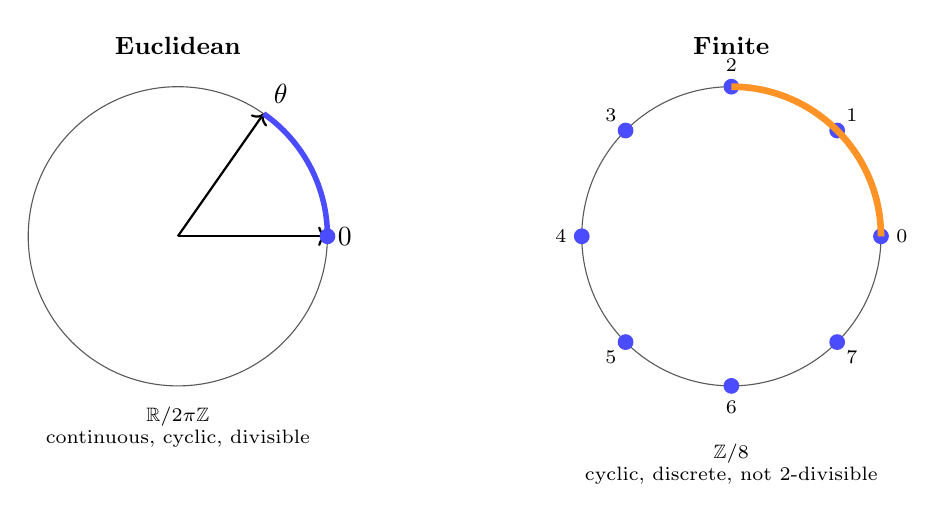
\begin{tikzpicture}[scale=0.95]
  % Euclidean
  \begin{scope}[xshift=-3.7cm]
    \draw[black!65] (0,0) circle (2);
    \draw[->, thick] (0,0)--(2,0) node[right] {$0$};
    \draw[->, thick] (0,0)--(55:2) node[above right] {$\theta$};
    \draw[blue!70, line width=2pt] (2,0) arc (0:55:2);
    \fill[blue!70] (2,0) circle (3pt);
    \node[font=\small\bfseries] at (0,2.55) {Euclidean};
    \node[font=\scriptsize,align=center] at (0,-2.55)
      {$\mathbb R/2\pi\mathbb Z$\\ continuous, cyclic, divisible};
  \end{scope}
  % finite
  \begin{scope}[xshift=3.7cm]
    \draw[black!65] (0,0) circle (2);
    \foreach \k in {0,...,7} {%
      \pgfmathsetmacro{\ang}{45*\k}%
      \fill[blue!70] (\ang:2) circle (3pt);%
      \node[font=\scriptsize] at (\ang:2.28) {\k};%
    }
    \draw[orange!85, line width=2.4pt] (2,0) arc (0:90:2);
    \node[font=\small\bfseries] at (0,2.55) {Finite};
    \node[font=\scriptsize,align=center] at (0,-3.05)
      {$\mathbb Z/8$\\ cyclic, discrete, not $2$-divisible};
  \end{scope}
\end{tikzpicture}
\end{document}
